% Clase
\documentclass[11pt,a4paper,spanish,twoside]{book}

% Órdenes auxiliares
% Español
\usepackage[spanish]{babel}
\usepackage[utf8]{inputenc}
\usepackage[T1]{fontenc}
\usepackage{lmodern}

% Imágenes
\usepackage[pdftex]{graphicx}
\usepackage{latexsym}
\usepackage{fancybox}

% Ruta para las imágenes
\graphicspath{{img/}}

% Rotaciones
\usepackage[twoside]{rotating}

% Multirow
\usepackage{multirow}

% Referencias
\usepackage[spanish]{varioref}
\usepackage[pdftex,colorlinks=true,linkcolor=black]{hyperref}

% Colores
\usepackage{color}
\usepackage{colortbl}

% Párrafos
\setlength{\parskip}{6pt}

% Code for creating empty pages
% No headers on empty pages before new chapter
\makeatletter
\def\cleardoublepage{\clearpage\if@twoside \ifodd\c@page\else
    \hbox{}
    \thispagestyle{empty}
    \newpage
    \if@twocolumn\hbox{}\newpage\fi\fi\fi}
\makeatother \clearpage{\pagestyle{empty}\cleardoublepage}

\usepackage{titlesec}

\titleformat{\chapter}[display]
  {\bfseries\Large}
  {\filleft\MakeUppercase{\chaptertitlename} \Huge\thechapter}
  {4ex}
  {\titlerule
   \vspace{2ex}%
   \filright}
  [\vspace{2ex}%
   \titlerule]

% Fancyhdr - Encabezados y pies de página
\usepackage{fancyhdr}
% Márgenes
\headsep=8mm
\footskip=14mm

% Fancy Header Style Options
\pagestyle{fancy}               % Sets fancy header and footer
\fancyfoot{}                    % Delete current footer settings

% Sin mayúsculas en la cabecera
\lhead{\nouppercase{\rightmark}}
\rhead{\nouppercase{\leftmark}}

% Capítulo
\renewcommand{\chaptermark}[1]{ % Lower Case Chapter marker style
  \markboth{\chaptername\ \thechapter.\ #1}{}} 

% Sección
\renewcommand{\sectionmark}[1]{ % Lower case Section marker style
  \markright{\thesection.\ #1}} 

% Página
\fancyhead[LE,RO]{\bfseries\thepage} % Page number (boldface) in left on even
                                     % pages and right on odd pages

% ------------------ Macro para encabezados y pies de página-------------------
%    Uso: \encabezado{pares(pag izquierda)}
% -----------------------------------------------------------------------------
\def\encabezado{
  \fancyhead[RE]{\bfseries\leftmark}     % In the right on even pages
  \fancyhead[LO]{\bfseries\rightmark}  % In the left on odd pages
  \renewcommand{\headrulewidth}{0.5pt} % Width of head rule
}
% -----------------------------------------------------------------------------

% ------------------ Macro para insertar una imagen ---------------------------
%    Uso: \imagen{nombreFichero}{Ancho(cm))}{Etiqueta}{Identificador}
% -----------------------------------------------------------------------------
\usepackage{float}
\usepackage{ifthen}
\def\imagen#1#2#3#4{
  \begin{figure}[H]
    \begin{center}
      \ifthenelse{\equal{#2}{}}
      {\includegraphics{#1}}{\resizebox{#2cm}{!}{\includegraphics{#1}}}
      \ifthenelse{\equal{#3}{}}{}{\caption{#3}}
      \label{#4}
    \end{center}
  \end{figure}
}
% -----------------------------------------------------------------------------


% ------------------ Macro para la portada ------------------------------------
%    Uso: \portada{asignatura}{titulo}{subtítulo}{autor}{fecha}
% -----------------------------------------------------------------------------
\def\portada#1#2#3#4#5{
  \thispagestyle{empty}
  \vspace*{-3.3cm}

  \begin{minipage}[t]{14cm}
    \begin{center}
      
\includegraphics[scale=0.25]{logoesi}
  
      \vspace*{1.5cm}
      {\Large \textbf{Universidad de Castilla-La Mancha\\ 
          Escuela Superior de Informática}\\}
    
      \vspace*{1.2cm}
      {\huge \textbf{#1}\\}
    
      \vspace*{1.5cm}
      {\huge #2}\\{\Large #3\\}
    
      \vspace*{1.5cm}
      {\large #4\\}
      \vspace*{1.4cm}
      \large{#5}
    \end{center}
  \end{minipage}

  \newpage
%   \vspace*{1cm}
%   \thispagestyle{empty} 
%   \newpage
}
% -----------------------------------------------------------------------------


% ------------------ Macro para la licencia -----------------------------------
%    Uso: \portada{asignatura}{titulo}{subtítulo}{autor}{fecha}
% -----------------------------------------------------------------------------
\def\licencia#1{
  \thispagestyle{empty}  % Suprime la numeración de esta página
  \vspace*{16.5cm}
  \begin{small}
    \copyright~ #1. Se permite la copia, distribución y/o 
    modificación de este documento bajo los términos de la licencia de
    documentación libre GNU, versión 1.1 o cualquier versión posterior publicada
    por la {\em Free Software Foundation}, sin secciones invariantes. Puede
    consultar esta licencia en http://www.gnu.org. \\[0.2cm]
    Este documento fue compuesto con \LaTeX{}. 
  \end{small}
  \newpage
%   \thispagestyle{empty}
%   \vspace*{0cm}
%   \newpage
}
% -----------------------------------------------------------------------------




% Encabezado y pie de página
\encabezado

\begin{document}

% Silabación extra
\hyphenation{
a-sig-na-tu-ras
au-to-ma-ti-za-rá
ca-li-dad
ca-tá-lo-go
ca-rre-ra
cons-truc-ción
co-rrec-ta-men-te
co-rres-pon-de
de-pen-dien-tes
de-sa-rro-llo
des-tru-yen
diag-nos-tico
dis-po-ni-bi-li-dad
fi-na-li-za-ción
ge-ne-ra-ción
in-fe-rior
man-te-ni-mien-to
me-ca-nis-mo
me-dian-te
o-cu-rren-cia
per-so-nal
pro-ce-di-mien-to
pro-ce-di-mien-tos
pro-por-cio-na-rá
pu-bli-ca-da
re-cha-zar
re-fe-ren-cia
re-lle-nar
re-qui-si-tos
res-pec-ti-va-men-te
res-pecto
res-pon-sa-bi-li-dad
u-su-a-rios
va-ria-rá
vi-lla-rre-al
}


% Portada
\portada{Ingeniería del Software}
{Práctica 2}{Diseño orientado a objetos}
{Sergio de la Rubia García-Carpintero\\Miguel Millán Sánchez-Grande\\
  Luis Muñoz Villarreal\\Alicia Serrano Sánchez\\
  Juan Miguel Torres Triviño}{28 de Mayo de 2010}

% Licencia
\licencia{Sergio de la Rubia García-Carpintero, Miguel Millán Sánchez-Grande,
  Luis Muñoz Villarreal, Alicia Serrano Sánchez, Juan Miguel Torres Triviño}

% Índices
\tableofcontents
%\listoftables
%\listoffigures

\chapter*{Prólogo}
El objetivo de la práctica es conocer y simular el ciclo de vida seguido
durante el desarrollo del software. Para ello se va a realizar un supuesto
práctico que incluye análisis de requisitos, diseño e implementación del
mismo. 

Dado que el enunciado fijado para la práctica no proporcionaba toda la
información necesaria para poder desarrollarla, se han realizado
una serie de entrevistas con el cliente para poder afianzar los requisitos
finales de la aplicación. Éstas reuniones son fundamentales para poder
conseguir un buen análisis e ir profundizando sobre las diferencias de las
ideas del cliente y las del equipo de síntesis y desarrollo del software, lo
que hace un paso imprescindible para un buen diseño y una buena implementación.

Además, al tratarse de un proyecto en grupo, proporciona habilidades en
nuestra formación como ingenieros, al tener que enfrentarse a un importante
aspecto de la vida real, el trabajo en equipo. Esto tiene partes positivas y
negativas, ya que al ser varios miembros se han de poner en común distintos
puntos de vista y llegar a un acuerdo para poder proseguir con el desarrollo;
pero también agiliza las etapas, ya que se pueden repartir las diferentes
tareas a realizar del trabajo. 

Con la realización de esta práctica se pretende conocer y asimilar los
objetivos básicos de la ingeniería del software: 
\begin{itemize}
\item Los procesos del ciclo de vida software y sus diferentes formas de
  organización en distintos modelos del ciclo de vida.
\item Los conceptos y actividades fundamentales del análisis de requisitos,
  así como su importancia en el desarrollo y mantenimiento del software.
\item Los conceptos, técnicas y diagramas básicos del paradigma de desarrollo
  orientado a objetos: desde el análisis a las pruebas.
\item Un modelo de proceso de aplicación del paradigma orientado a objetos, que
  incluya el proceso de análisis, diseño y estrategias de prueba.
\item Las posibilidades que ofrece la reutilización del software en todos los
  niveles de desarrollo.
\end{itemize}

\part{Análisis}
\chapter{Especificación de requisitos}
\section{Requisitos iniciales del sistema}
Se desarrolla una aplicación para la gestión distribuída de la
revisión de proyectos de investigación, además de prestar soporte para
distintas solicitudes (becas, acciones integradas, etc.). El sistema lo
mantiene una agencia de evaluación de proyectos, que es la encargada
de ofrecer una valoración de los proyectos de investigación que le envían
distintos organismos (ministerios, comunidades autónomas, etc.). Existe un
conjunto de áreas temáticas y cada área está compuesta por un conjunto de
subáreas. Cada área tiene un \emph{coordinador}, que se encarga de asignar
proyectos a cada uno de los \emph{adjuntos} de cada subárea. El
\emph{adjunto} se encargará de asignar la evaluación de sus proyectos a los
expertos más adecuados y de, finalmente, realizar los informes finales de
evaluación. El sistema es utilizado por los siguientes tipos de usuario: 

\begin{itemize}
\item Los \emph{expertos} realizan evaluaciones de proyectos. Reciben una 
  invitación que pueden aceptar o declinar. Una vez que los expertos aceptan
  la invitación, tendrán un tiempo determinado para enviar sus informes. 
\item Los \emph{adjuntos} realizan asignaciones de proyectos a
  \emph{expertos}. También tienen la funcionalidad de desasignar a
  \emph{expertos} o insistir si el experto tarda demasiado en la realización
  de un informe. Una vez recibidos los informes de los \emph{expertos}, el
  adjunto realiza un único informe final, que se devuelve a la entidad
  solicitante una vez validado por el \emph{coordinador} del área
  correspondiente.     
\item Los \emph{coordinadores} asignan proyectos a los \emph{adjuntos} y
  realizan la supervisión de todos los informes. 
\item El \emph{secretario} de la agencia de evaluación carga en el sistema todos
  los documentos de los proyectos (memoria del proyecto, currículum de los
  investigadores, texto de la convocatoria, etc.). 
\end{itemize}

\section{Análisis de requisitos del sistema}
Tras una serie de reuniones, los requisitos finales del sistema son
los siguientes: 

\subsection{Usuarios}
\begin{itemize}
\item Acceden al sistema mediante un identificador, que será el dni; y una 
contraseña, que se podrá modificar.
\item Hay cuatro tipos: secretario, coordinador, adjunto y experto. Cada uno
  con diferente funcionalidad y rango. 
\item Cada usuario podrá modificar sus datos personales y tendrá una vista
  restringida sobre la lista de proyectos dependiendo de su rango en el 
  sistema.
\end{itemize}

\subsection{Paquete de proyectos}
Las instituciones solicitantes mandan los proyectos en paquetes al
secretario, los cuales contienen: 
\begin{itemize}
\item La convocatoria, que describe uno o varios modelos de
  evaluación. Estos a su vez contienen los criterios para evaluar cada
  proyecto del paquete.

\item Las bases del proyecto.

\item La institución convocante.

\item Los proyectos, que opcionalmente pueden venir clasificados por área. 

\item Cada proyecto tendrá un plazo estipulado para que la evaluación esté
  realizada. 
\end{itemize}

\subsection{Secretario}
\begin{description}
\item[Usuarios] Es el encargado de añadir, modificar y eliminar 
  usuarios del sistema (coordinadores, adjuntos y expertos).
\item[Coordinadores] Elegirá el coordinador de cada área.
\item[Paquetes de proyecto] Recibe las solicitudes de evaluación de proyectos
  en forma de paquetes de proyectos y los introduce al sistema (las bases, la
  convocatoria, la institución convocante, los proyectos - los cuales serán
  asignados a un área -, \dots). También podrá modificar cualquier información
  referente a estas solicitudes.  
\item[Modelos de evaluación] Dependiendo de la información que contenga el
  proyecto, elaborará unos modelos de evaluación. 
\item[Plazos expertos] Decidirá los plazos que tienen los expertos para
  aceptar o declinar la invitación para realizar el informe de evaluación,
  y una vez aceptada, la fecha para entregar dicho informe.
\end{description}

\subsection{Coordinador}
\begin{itemize}
\item Pertenece a una única área.
\item Establece las subáreas de los proyectos que se le asignan.
\item Dentro de su área asigna un adjunto a cada subárea.
\item Reasigna un proyecto a otra subárea, si el adjunto se lo indica.
\item Valida los informes pendientes que los adjuntos de su correspondiente 
  área realizan.
\end{itemize}

\subsection{Área}
\begin{itemize}
\item Está asociada a un único coordinador y tiene, a su vez, varias subáreas. 
\item El número de subáreas podrá ser diferente en cada área.
\end{itemize}

\subsection{Adjunto}
\begin{itemize}
\item Pertenece únicamente a una subárea.
\item Tiene una serie de proyectos asignados.
\item Busca a los expertos especificando el área, la institución, palabras
  clave y valoraciones, en las que se prioriza la formalidad de plazos y
  calidad de las evaluaciones. 
\item Una vez finalizada la búsqueda, elige a uno o más expertos, según
  considere necesario, y les envía un modelo de invitación predeterminado
  mediante correo electrónico para la evaluación del proyecto.  
\item Puede reasignar las evaluaciones si el experto declina la invitación,
  no obtiene respuesta dentro del plazo o si el experto no cumple con los
  plazos de entrega del informe de evaluación.
\item El adjunto puede insistir a los expertos correspondientes cuando esté
  próxima la fecha límite de entrega del informe de evaluación.
\item Una vez realizada las evaluaciones de los expertos, el adjunto
  realiza un informe final teniendo en cuenta los informes de los distintos
  expertos que hayan aceptado realizar la evaluación. Este informe final
  debe ser validado por el coordinador de su área. 
\item Evalúa el trabajo del experto basándose en la formalidad de los plazos
  y la calidad de su informe. 
\item Puede recomendar al secretario añadir expertos.
\item Dentro de la lista de proyectos a las que los adjuntos tienen acceso,
  tiene una sublista de los expertos que están realizando la evaluación de
  ese proyecto.  
\item Puede avisar al coordinador cuando el proyecto no corresponda a su
  subárea. 
\end{itemize}

\subsection{Subárea}
\begin{itemize}
\item Sólo puede pertenecer a un área y tiene un único adjunto asociado.
\end{itemize}

\subsection{Expertos}
\begin{itemize}
\item Pueden tener asignados varios proyectos a la vez. 
\item No pueden pertenecer a la misma institución solicitante de la evaluación.
\item Pueden aceptar o declinar las invitaciones de evaluación de proyectos.
\item Cuando acepte la invitación, pueden acceder a la documentación de ese
  proyecto e ir realizando progresivamente el informe en varias sesiones. 
\item Una vez que terminen el informe finalizan el proceso de evaluación.
\item Reciben avisos de finalización de plazos por parte del adjunto para
  finalizar el informe, vía correo electrónico.
\item Cada uno tiene una serie de palabras clave asociadas a su
  temática. Éstas palabras clave se utilizan como parámetros en las
  búsquedas. 
\item Tienen una lista de evaluaciones pendientes, que pueden aceptar o 
  rechazar.
\item El sistema avisa de los plazos que tiene el experto para aceptar o
  declinar una invitación. Además, una vez aceptada dicha invitación, se le
  comunican los plazos de entrega del informe de evaluación, según definió
  el secretario.

\end{itemize}

\chapter{Diagrama de casos de uso}
Un \emph{caso de uso} es una técnica para la captura de requisitos
potenciales de un nuevo sistema o una actualización de software. Cada caso de
uso proporciona uno o más escenarios que indican cómo debería interactuar el
sistema con el usuario o con otro sistema para conseguir un objetivo
específico. En ocasiones, se utiliza a usuarios sin experiencia junto a los
analistas para el desarrollo de casos de uso.

En otras palabras, un caso de uso es una secuencia de interacciones que se
desarrollan entre un sistema y sus actores en respuesta a un evento que
inicia un actor principal sobre el propio sistema. Los diagramas de casos de
uso sirven para especificar la comunicación y el comportamiento de un sistema
mediante su interacción con los usuarios y/u otros sistemas. Los diagramas de
casos de uso se utilizan para ilustrar los requerimientos del sistema al
mostrar cómo reacciona a eventos que se producen en su ámbito o en él mismo.

La \emph{figura \ref{dcasouso}} muestra el diagrama de casos de uso del
sistema.
\imagen{Casos.png}{15.5}{Diagrama de casos de uso del sistema GDRPI}{dcasouso}


\chapter{Diagramas de secuencia}
Un \emph{diagrama de secuencia} muestra la interacción de un conjunto de
objetos en una aplicación a través del tiempo y se modela para cada método de
la clase. Mientras que el \emph{diagrama de casos de uso} permite el modelado
de una vista \emph{business}\footnote{Vista génerica de la implementación del
escenario, no contiene detalles específicos.} del escenario, el diagrama de 
secuencia contiene detalles de implementación del escenario, incluyendo los 
objetos y clases que se usan para implementar el escenario, y mensajes 
intercambiados entre los objetos.

Típicamente uno examina la descripción de un caso de uso para determinar qué
objetos son necesarios para la implementación del escenario. Un diagrama de 
secuencia muestra los objetos que intervienen en el escenario con líneas 
discontinuas verticales, y los mensajes pasados entre los objetos como
flechas horizontales.

\section{Entrada al sistema}
La vista inicial del sistema, muestra una pantalla en la que se pide el nombre
de usuario y la contraseña. Para autentificarse, el usuario debe rellenar
estos campos y pulsar el botón ``Entrar''. El sistema recoge los datos y los
comprueba con los existentes en una tabla de la base de datos que contiene los
datos de todos los usuarios. En caso de haber correspondencia (caso reflejado
en el diagrama de la \emph{figura \ref{EntSisCor}}), el usuario podrá
visualizar la interfaz correspondiente a su rango dentro del sistema. En caso
de no haberla (como muestra la \emph{figura \ref{EntSisErr}}), el sistema 
mostrará el mensaje: ``usuario o contraseña incorrectas''.

\imagen{EntSisCor.png}{13}{Entrada al sistema correcta}
{EntSisCor}
\imagen{EntSisErr.png}{13}{Entrada al sistema errónea}
{EntSisErr}

\section{Secretario introduce paquete de proyectos}
Se parte de la base de que el secretario se ha autentificado en el sistema y
tiene acceso a la vista general del secretario.

La vista general del secretario accede al sistema para proporcionar una
lista con los paquetes de proyectos introducidos anteriormente. En este caso
el secretario le da a ``Introducir nuevo paquete'' y completa los campos
pertinentes para identificarlo. Una vez completada la operación, el
coordinador acepta y el sistema almacena el nuevo paquete vacío y actualiza
la lista mostrada de paquetes de proyectos. A continuación, el secretario
marca el paquete creado y selecciona la opción de ``Introducir nuevo 
proyecto''. Uno a uno empieza a introducir los proyectos que forman parte del
paquete y el sistema los va almacenando.

Ahora el secretario se dispone a consultar la información de un paquete.
Para ello selecciona un paquete y le da a la opción de ``Modificar''. El
sistema carga la información almacenada acerca del paquete y la muestra
incluyendo los proyectos asociados a dicho paquete.

El diagrama de secuencia de este escenario se muestra en la \emph{figura
\ref{SecIntPaq}}.

\imagen{SecIntPaq.png}{13}{Secretario
introduce un paquete de proyectos y consulta su contenido}{SecIntPaq}

\section{Secretario crea un modelo de evaluación}
Se parte de la base de que el secretario se ha autentificado en el sistema y
tiene acceso a la vista general del secretario.

El secretario selecciona la pestaña de ``Modelos de evaluación''. A
continuación, el sistema le proporciona una vista con los paquetes de
proyectos existentes. El secretario pulsa la opción de ``Añadir'' y el sistema
le muestra una estructura vacía y le da acceso a seleccionar uno de los
paquetes de proyectos. A continuación, el secretario selecciona el paquete de
proyectos que contendrá el modelo de evaluación que se dispone a realizar.
El secretario va añadiendo elemento a elemento a la estructura y el sistema
va actualizando la vista actual de la estructura. Finalmente, el secretario
almacena en la base de datos el modelo de evaluación seleccionando la opción
``Guardar''.

El diagrama de secuencia de este escenario se muestra en la \emph{figura
\ref{SecCreMod}}.

\imagen{SecCreMod.png}{13}{Secretario crea un
modelo de evaluación}{SecCreMod}

\section{Coordinador selecciona experto para ser adjunto}
Se parte de la base de que el coordinador se ha autentificado en el sistema y
tiene acceso a la vista general del coordinador.

El coordinador selecciona la pestaña de ``Subáreas''. A continuación, el
sistema le proporciona una vista con las subáreas existentes en el área a la
que pertenece. El coordinador marca la subárea que cambiará de adjunto y
selecciona la opción de ``Búsqueda de expertos''. Establece una serie de
parámetros de búsqueda y confirma la búsqueda. El sistema realiza una búsqueda
en su base de datos con los parámetros especificados y devuelve una lista
con los expertos encontrados. Por último, el coordinador marca a uno de los
expertos y lo confirma como nuevo adjunto de la subárea. El sistema cambia
el rango del usuario experto por el de adjunto y lo asigna a la subárea
elegida.

El diagrama de secuencia de este escenario se muestra en la \emph{figura
\ref{CooExpAdj}}.

\imagen{CooAdjSub.png}
{13}{Coordinador selecciona a un experto para ser adjunto de una subárea}
{CooExpAdj}

\section{Coordinador asigna un proyecto a una subárea}
Se parte de la base de que el coordinador se ha autentificado en el sistema y
tiene acceso a la vista general del adjunto.

La vista general del coordinador accede al sistema para proporcionar una
lista con los proyectos asociados a su área. A continuación, el coordinador
marca uno de los proyectos y selecciona la opción de ``Asignar subárea''. El
sistema realiza una búsqueda de las subáreas que pertenecen al área del
coordinador y devuelve por pantalla una lista con estas. Finalmente, el
coordinador marca una de las subáreas de la lista y confirma la asignación
al sistema. El sistema asigna entonces el proyecto a dicha subárea.

El diagrama de secuencia de este escenario se muestra en la \emph{figura
\ref{CooProSub}}.

\imagen{CooProSub.png}
{13}{Coordinador asigna un proyecto a una subárea}{CooProSub}

\section{Coordinador valida informe}
Se parte de la base de que el coordinador se ha autentificado en el sistema y
tiene acceso a la vista general del adjunto.

La vista general del coordinador accede al sistema para proporcionar una
lista con los proyectos asociados a su área. El coordinador marca uno
de los proyectos y selecciona la opción de ``Ver/Modificar'' el informe del
proyecto. El sistema carga el informe del proyecto realizado por el adjunto
y la documentación asociada a este. Una vez conformado con el informe del
adjunto, el coordinador le da a ``Validar informe'', entonces el sistema
cambia el estado del informe a ``evaluado''.

El diagrama de secuencia de este escenario se muestra en la \emph{figura
\ref{CooValInf}}.

\imagen{CooValInf.png}{13}{Coordinador valida informe de
evaluación}{CooValInf}

\section{Adjunto busca expertos para evaluar proyecto}
Se parte de la base de que el adjunto se ha autentificado en el sistema y
tiene acceso a la vista general del adjunto.

La vista general del adjunto accede al sistema para proporcionar una lista
con los proyectos asociados a su subárea. El adjunto selecciona uno de los
proyectos de la lista y utiliza la funcionalidad de buscar experto. La 
interfaz le muestra un campo para que el adjunto introduzca los parámetros de
búsqueda de expertos. Una vez introducidos, el adjunto da la señal de
aceptar la búsqueda. El sistema utiliza los parámetros para iniciar una 
búsqueda con los expertos que tiene almacenados en la base de datos. La
búsqueda finaliza devolviento una lista con los expertos que contienen las
palabras clave. Por último, el adjunto selecciona los expertos que desea que
evalúen el proyecto y acepta la selección para que el sistema elabore y
envíe una invitación personalizada de evaluación para cada uno de estos
expertos.

El diagrama de secuencia de este escenario se muestra en la \emph{figura
\ref{AdjBusExp}}.

\imagen{AdjBusExp.png}{13}
{Adjunto busca expertos para evaluar proyecto}{AdjBusExp}

\section{Adjunto realiza informe}
Se parte de la base de que el adjunto se ha autentificado en el sistema y
tiene acceso a la vista general del adjunto.

La vista general del adjunto accede al sistema para proporcionar una lista
con los proyectos asociados a su subárea. El adjunto marca el símbolo ``+''
de uno de los proyectos de la lista y el sistema le muestra una lista de 
expertos que están evaluando el proyecto. A continuación, marca a uno de los
expertos y el sistema accede al informe realizado por dicho experto. Después
de consultar el informe, el adjunto selecciona la opción de ``Realizar
informe''. El sistema consulta el modelo de evaluación que tiene asignado el
proyecto y lo muestra por pantalla. El adjunto modificará varias veces
el contenido del informe y finalmente lo confirmará mediante la opción de
``Finalizar informe''. El sistema entonces cambiará el estado del proyecto a
``evaluado por el adjunto''.

El diagrama de secuencia de este escenario se muestra en la \emph{figura
\ref{AdjReaInf}}.

\imagen{AdjReaInf.png}{13}{Adjunto realiza informe de evaluación}
{AdjReaInf}

\section{Experto realiza informe}
Se parte de la base de que el experto se ha autentificado en el sistema y
tiene acceso a la vista general del experto.

El experto solicita al sistema la lista de proyectos que tiene asignados. El
sistema accede a una tabla en la base de datos, que relaciona los expertos con
los proyectos que tiene asignados y le devuelve por pantalla una lista con 
estos. A continuación, el experto selecciona uno de los proyectos de la lista
y el sistema recupera la información asociada a este, así como de haberlo, el
informe realizado por el experto sobre el proyecto. Después, el experto
redacta el informe conforme al modelo que este sigue y guarda y finaliza su
edición. Finalmente, El sistema almacena dicho informe y cambia su estado a
``finalizado''.

El diagrama de secuencia de este escenario se muestra en la \emph{figura
\ref{ExpReaInf}}.

\imagen{ExpReaInf.png}{13}{Experto realiza informe de evaluación}
{ExpReaInf}

\part{Diseño}
\chapter{Diagrama de clases}
Un \emph{diagrama de clases} es un tipo de diagrama estático que describe la
estructura de un sistema mostrando sus clases, atributos y las relaciones
entre ellos. Los diagramas de clases son utilizados durante el proceso de
diseño de los sistemas, donde se crea el diseño conceptual de la
información que se manejará en el sistema, y los componentes que se
encargarán del funcionamiento y la relación entre uno y otro.

Al diseñar una clase se debe pensar en cómo se puede identificar un objeto
real, como una persona, un transporte, un documento o un paquete. Estos
ejemplos de clases de objetos reales son sobre lo que un sistema se
diseña. Durante el proceso del diseño de las clases se toman las propiedades
que identifican como único al objeto y otras propiedades adicionales como
datos que corresponden al objeto. El diagrama de clases incluye mucha más
información como la relación entre un objeto y otro, la herencia de
propiedades de otro objeto y conjuntos de operaciones/propiedades que son
implementadas para una interfaz.

La \emph{figura \ref{dclases}} muestra el diagrama de clases del sistema.

\begin{sidewaystable}
\begin{figure}[H]
  \begin{center}
    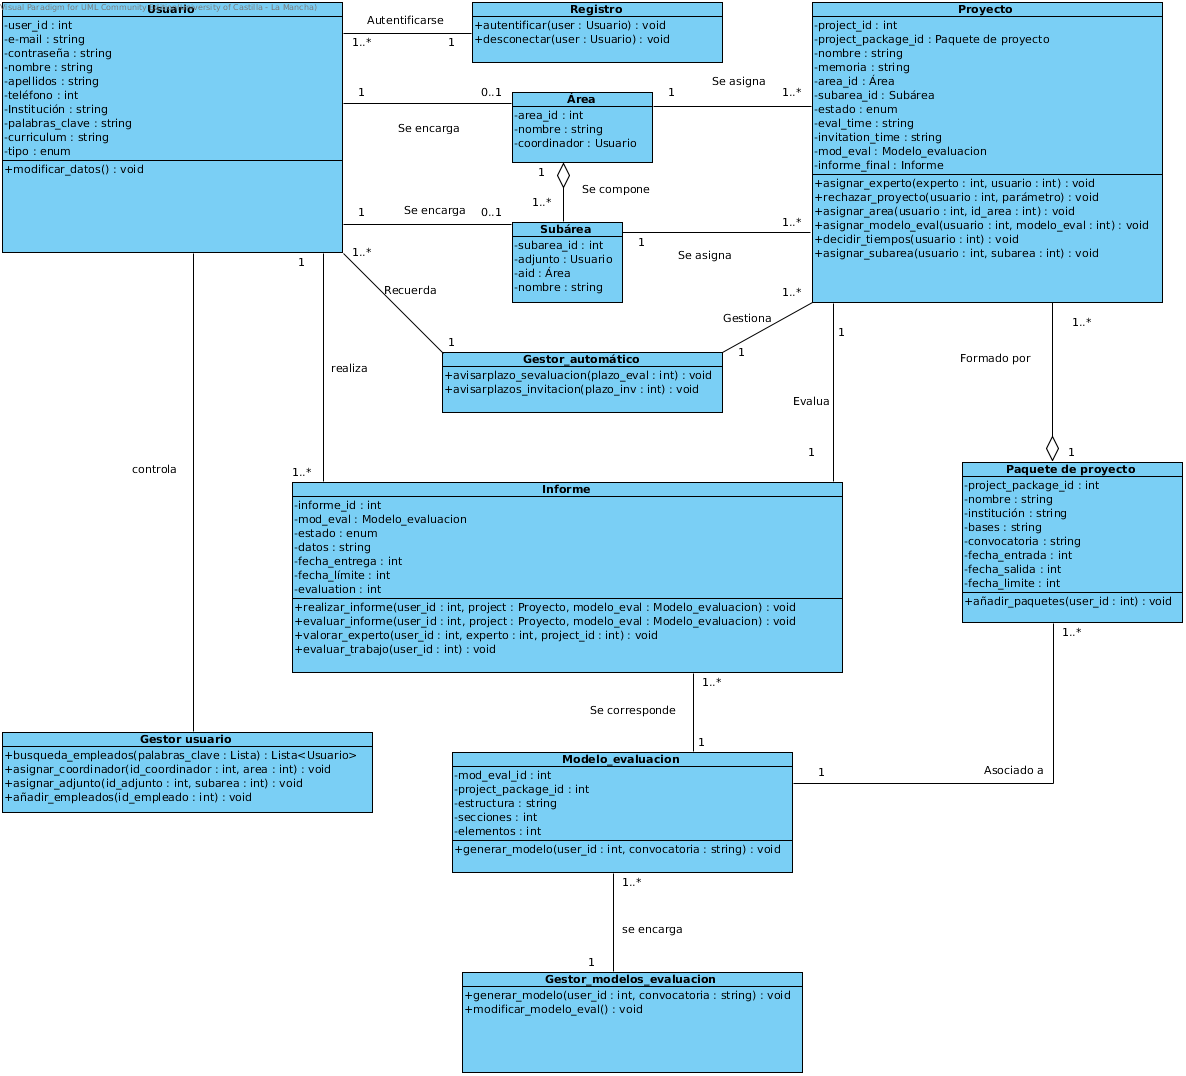
\includegraphics[scale=0.6]{Clases.png}
    \caption{Diagrama de clases}
    \label{dclases}
  \end{center}
\end{figure}
\end{sidewaystable}
\chapter{Diagrama relacional}
Es el modelo más utilizado en la actualidad para modelar problemas reales y 
administrar datos dinámicamente.

Se trata de un modelo lógico que establece una estructura sobre los datos,
aunque posteriormente éstos puedan ser almacenados de múltiples formas (con
el objetivo de aprovechar las características físicas concretas de la máquina
sobre la que se implante la base de datos realmente).

El diagrama relacional del sistema \emph{GDRPI} se representa en la
\emph{figura \ref{drel}}.

\imagen{MRE.pdf}{13}{Diagrama Relacional}{drel}

\part{Implementación}
\chapter{Manual de usuario}
\section{Introducción}
La Gestión Distribuída de la Revisión de Proyectos de Investigación es una
aplicación web que incluye todo lo necesario para conseguir una comunicación 
activa entre el usuario y la información que puede manejar. Cada usuario podrá 
manejar diferentes acciones según el rango que tenga en la empresa (secretario,
coordinador, adjunto o experto).

La implementación de la práctica incluye todo lo relacionado con la gestión de
las e\-va\-lua\-cio\-nes. Entre las diferentes posibilidades de la aplicación se
encuentran: la realización de modelos de evaluación, la asignación de proyectos
a expertos, la realización de informes de evaluación, la modificación de
informes de evaluación, la eliminación de informes de evaluación, la consulta
de informes de evaluación y el envío de informes de evaluación a la institución
convocante. 

\section{Inicio de sesión}
La pantalla de inicio de la aplicación se puede observar en la figura
\ref{img1} de la página \pageref{img1}.

\imagen{acceso.pdf}{13}{\small{Acceso a la aplicación.}}{img1}

\begin{itemize}
\item Se introduce el usuario y la contraseña proporcionados en el correo de 
alta (figura \ref{img2}, página \pageref{img2}).

\imagen{introducirdatos.pdf}{4}{\small{Datos del usuario.}}{img2}

\item Si los datos son incorrectos, no se puede acceder a la aplicación y se
  muestra un mensaje de error. 
\end{itemize}

La página inicial para cada tipo de usuario muestra la información 
co\-rres\-pon\-dien\-te a las funciones que puede realizar con respecto a las 
evaluaciones de informes.


\section{Secretario}
\subsection{Crear un modelo de evaluación}
\begin{enumerate}
\item Pulsar ``Añadir'' para agregar un nuevo modelo de evaluación, como se 
  puede ver en la página \pageref{sc1}, en la figura \ref{sc1}. Se despliegan
  los datos que se pueden introducir en un modelo de evaluación.
  
  \imagen{anadirmod.pdf}{10}{Añadir modelo de evaluación.}{sc1}

\item Ver convocatoria de un paquete de proyectos.
  \begin{itemize}
  \item En la sección CONVOCATORIAS se despliega una lista (figura \ref{sc2}) 
    donde se puede elegir el paquete de proyectos del que se desea ver la 
    convocatoria.

    \imagen{convmod.pdf}{10}{\small{Elección de paquete de
        proyectos.}}{sc2}

  \item Se elige un paquete de proyectos y se pulsa ``Ver''. A la derecha de la 
    página se muestra la información de la convocatoria (figura \ref{sc3},
    página \pageref{sc3}).

    \imagen{convmostrada.pdf}{13}{\small{Información de
        convocatoria.}}{sc3}
  \end{itemize}

\item Agregar los tipos de elementos de la sección FORMULARIOS pulsando 
  ``Añadir'', como se puede observar en la figura \ref{sc4} de la página
  \pageref{sc4}. En la sección 
  \emph{Estructura} se muestra el resultado del modelo de evaluación que se
  está creando.

  \imagen{formularios.pdf}{4}{\small{Opciones de modelos de
      evaluación.}}{sc4}

\item Guardar el modelo de evaluación realizado. Para ello se pulsa el botón 
  ``Guardar'' que está situado al final de la sección FORMULARIOS.
\end{enumerate}

\subsection{Modificar o eliminar un modelo de evaluación}
Se marca el paquete de la convocatoria que se desea modificar y se pulsa 
``Modificar'' o ``Eliminar'' según se desee (figura \ref{img7}).
\imagen{modifmod.pdf}{14}{\small{Modificación y eliminación de un modelo.}}
{img7}

\section{Coordinador}
La pantalla principal del coordinador muestra las posibles acciones a realizar 
(figura \ref{c1}, página \pageref{c1}).
\imagen{corprinc.pdf}{13}{\small{Ventana Principal del coordinador.}}{c1}

\subsection{Ver/Modificar informe final}
\begin{enumerate}
\item Se selecciona el proyecto deseado de entre los disponibles (figura 
  \ref{c2}, página \pageref{c2}). Los proyectos asignados se muestran en una
  tabla.
  
  \imagen{selcor.pdf}{13}{\small{Selección de proyecto.}}{c2}

\item Para consultar o modificar el informe final, pulsar 
  ``Ver/Modificar informe'' y se expande el correspondiente modelo de 
  evaluación (figura \ref{c3}, página \pageref{c3}).

  \imagen{modinf.pdf}{13}{\small{Ver/modificar el informe final.}}{c3}

\item El botón ``Guardar'' permite guardar los cambios y editar en 
  posteriores sesiones, mientras que el botón ``Finalizar'' dar por finalizado 
  el informe (figura \ref{c4}, página \pageref{c4}).
  
  \imagen{opcor.pdf}{13}{\small{Guardar o finalizar informe final.}}{c4}
\end{enumerate}

\subsection{Validar informe final}
Se selecciona el proyecto deseado y se pulsa ``Validar informe final'', como se 
puede ver en la figura \ref{c5}, en la página \pageref{c5}.
\imagen{valinf.pdf}{13}{\small{Validación informe final.}}{c5}

\section{Adjunto}
La pantalla de inicio correspondiente se puede ver en la figura \ref{a1} de
la página \pageref{a1}.
\imagen{adjprinc.pdf}{13}{\small{Ventana Principal del adjunto.}}{a1}

\subsection{Asignar expertos}
\begin{itemize}
\item Se selecciona un determinado proyecto mostrado en la vista del adjunto y
  se pulsa ``Asignar expertos''.
\item A continuación, se despliega la información de los expertos que están
  asignados en ese proyecto junto con la información del estado del informe de
  cada experto.
\item Para buscar expertos, se muestra los determinados campos para realizar una
  búsqueda avanzada (figura \ref{busexp}, pág.\ref{busexp}). Los campos de los
  que consta la búsqueda son \emph{Nombre}, \emph{Apellidos}, \emph{Palabras
    clave}, \emph{Institución}, \emph{Nº de proyectos} y \emph{Valoración}. 
\imagen{busexp.png}{13}{Vista de búsqueda de expertos del adjunto}{busexp}
\item Se puede rellenar cualquier campo para realizar la búsqueda y la
  aplicación da el resultado en forma de lista, como se puede observar en la
  figura \ref{resexp} de la página \pageref{resexp}.
\imagen{resexp.png}{13}{Vista del resultado de la búsqueda de
expertos}{resexp}
\item Seleccionar un experto y pulsar ``Asignar''.
\end{itemize}

\subsection{Realizar informe final}
\begin{enumerate}
\item Se selecciona el proyecto deseado de entre los disponibles (figura 
  \ref{a2}, página \pageref{a2}). Los proyectos asignados se muestran en
  una tabla.
  
  \imagen{seladj.pdf}{13}{\small{Selección de proyecto.}}{a2}

\item Pulsando la opción ``+'', que aparece en la columna Exps, se puede ver qué
  expertos han realizado evaluaciones sobre el proyecto, como se puede ver en
  la figura \ref{a3} de la página \pageref{a3}. 

  \imagen{listaexp.pdf}{13}{\small{Expertos del proyecto seleccionado.}}{a3}

\item Pulsando el icono de consulta, se puede acceder a la evaluación realizada 
  por cada uno de los expertos (figura \ref{a4}, página \pageref{a4}).

  \imagen{coneval.pdf}{13}{\small{Consulta evaluación.}}{a4}

\item Para realizar el informe final, se pulsa ``Realizar informe'' 
  para que se expanda el correspondiente modelo de evaluación (figura
  \ref{a5}, página \pageref{a5}).
  
  \imagen{inffinal.pdf}{13}{\small{Realización informe final.}}{a5}

\item El adjunto puede ``Guardar'' o ``Finalizar informe'' 
  (figura \ref{a6}, página \pageref{a6}), el primero nos permite guardar
  los cambios y editar en posteriores sesiones, mientras que el segundo
  finaliza el informe.
  
  \imagen{opinf.pdf}{11}{\small{Guardar o finalizar informe final.}}{a6}
\end{enumerate}

\subsection{Valorar Experto}

\begin{itemize}
\item Se selecciona un proyecto y se pulsa la opción ``+'', que aparece en la
  columna Exps. A continuación, se muestra los expertos que han realizado
  evaluaciones sobre el proyecto.
\item Se selecciona un determinado experto y se pulsa ``Valorar experto''. Se
  expande un área de texto donde se introduce un comentario sobre el trabajo
  realizado; y también un campo donde se introduce la valoración numérica del
  experto. Para más detalle ver figura \ref{valexp} de la página
  \pageref{valexp}. 
\imagen{valexp.png}{11}{Vista de valoración de los expertos}{valexp}
\end{itemize}

\section{Experto}
\subsection{Realizar evaluación de un proyecto}
\begin{enumerate}
\item Los proyectos asignados se muestran en una tabla. Para realizar la 
  evaluación de un proyecto, se marca y se pulsa ``Realizar evaluación''
  (figura \ref{img8}, página \pageref{img8}). 

  \imagen{realizareval.pdf}{13}{\small{Elegir proyecto para
      evaluación.}}{img8}

\item Se expande el correspondiente modelo de evaluación, mostrando los 
  diferentes puntos a evaluar. En la parte izquierda de la pantalla se
  muestra la memoria de dicho proyecto, como se puede ver en la figura
  \ref{img9} de la página \pageref{img9}. 

  \imagen{evalexp.pdf}{13}{\small{Realización de evaluación.}}{img9}

\item Se guardan los cambios realizados en la evaluación con el botón 
  ``Guardar'' o se finaliza la evaluación pulsando ``Finalizar''.
\end{enumerate}

\chapter{Implementación}
\section{Introducción}
Para llegar a este punto de la práctica, se han seguido una serie de pautas de
planificación y diseño para conseguir una implementación eficiente y viable.
Con el objetivo de cumplir las necesidades del cliente se han utilizado los
siguientes lenguajes:
\begin{itemize}
\item PHP\cite{achour}: lenguaje de cuarta generación que genera páginas de cara
al servidor.
\item XHTML\cite{wc}: encargado de la información y la estructura de la página.
\item MySQL: se utiliza en el diseño e implementación de la base de datos.
\item CSS\cite{wc}: encargado de la maquetación y el estilo del modelado.
\item JavaScript\cite{resig}: empleado en el \emph{framework jQuery} da 
dinamismo al navegador.
\end{itemize} 
El objetivo es conocer el ámbito de aplicación de los servicios web, comprender 
y diseñar arquitecturas orientadas a servicios. Además, conocer los estándares y
los organismos de estandarización, conocer y aplicar técnicas de modelado y 
especificación de procesos, y servicios web complejos.

\section{Código fuente}
\subsection{index.php}
%\lstinputlisting[language=PHP]{../GDRPI/index.php}

\subsection{settings.php}
%\lstinputlisting[language=PHP]{../GDRPI/settings.php}

\subsection{js/main.js}
%\lstinputlisting[language=PHP]{../GDRPI/js/main.js}

\subsection{js/models.js}
%\lstinputlisting[language=PHP]{../GDRPI/js/models.js}

\subsection{js/projects.js}
%\lstinputlisting[language=PHP]{../GDRPI/js/projects.js}

\subsection{js/reports.js}
%\lstinputlisting[language=PHP]{../GDRPI/js/reports.js}

\subsection{inc/html.php}
%\lstinputlisting[language=PHP]{../GDRPI/inc/html.php}

\subsection{inc/loginout.php}
%\lstinputlisting[language=PHP]{../GDRPI/inc/loginout.php}

\subsection{inc/modelmanager.php}
%\lstinputlisting[language=PHP]{../GDRPI/inc/modelmanager.php}

\subsection{inc/mysql.php}
%\lstinputlisting[language=PHP]{../GDRPI/inc/mysql.php}

\subsection{inc/projectmanager.php}
%\lstinputlisting[language=PHP]{../GDRPI/inc/projectmanager.php}

\subsection{inc/reportmanager.php}
%\lstinputlisting[language=PHP]{../GDRPI/inc/reportmanager.php}

\subsection{inc/user.php}
%\lstinputlisting[language=PHP]{../GDRPI/inc/user.php}

\subsection{css/login.css}
%\lstinputlisting[language=PHP]{../GDRPI/css/login.css}

\subsection{css/main.css}
%\lstinputlisting[language=PHP]{../GDRPI/css/main.css}

\subsection{css/models.css}
%\lstinputlisting[language=PHP]{../GDRPI/css/models.css}

\subsection{css/reports.css}
%\lstinputlisting[language=PHP]{../GDRPI/css/reports.css}

\subsection{css/users.php}
%\lstinputlisting[language=PHP]{../GDRPI/css/users.php}

\appendix
\chapter{Carga de trabajo}
\begin{center}
  \begin{tabular}{p{10cm}|c}
    \textbf{Apellidos y Nombre} & \textbf{Porcentaje} \\ \hline \hline
    de la Rubia García-Carpintero, Sergio & 28\% \\
    Millán Sánchez-Grande, Miguel         & 18\% \\ 
    Muñoz Villarreal, Luis                & 18\% \\ 
    Serrano Sánchez, Alicia               & 18\% \\ 
    Torres Triviño, Juan Miguel           & 18\% \\
  \end{tabular}
\end{center}

\bibliographystyle{plain} 
\bibliography{iso2}

\end{document}
